\documentclass[main.tex]{subfiles}

\begin{document}

\section{Testing Methodology} \label{sec:results:method}

Measurements were done only in the algorithmic section of the program, disregarding any input and output operations as well as initial setup of \starpu and other libraries. All implemented approaches (\cpu, \gpu and the multiple \starpu options) were analysed, with the first two serving mostly for comparison with the framework.

In the main rendering loop, the time for each full iteration of the SPPMPA algorithm was measured (see \cref{fig:diagram_cpu}, which explains how iterations are organized). This was done by obtaining the time-stamp at the beginning of each iteration, and at the end of the last task of the same iteration, which also works well when using concurrent iterations. The full iteration time includes the required data transfer times, but more granular values were obtained, by measuring the time for each invoked task of each iteration, which does not account for data transfers. Presented results show only the average time of each iteration for the execution (with at least 100 iterations each). Full calibration was done prior to any \starpu test (except the calibration test shown in \cref{sec:prof:calibration}).
Since support for concurrent iterations was not fully implemented until later in the development stages, most results focus only on the approach of using only a single iteration at a time.

Since the entire main loop consists solely on task invocations, it was assumed that the difference between total iteration time and the sum of each task within the iteration corresponds to idle periods when the framework is waiting for resources or dependencies, or performing data transfers.

For each measurement, only the time spent in the main rendering function was considered, discarding any input and output time spent by the program. A minimum of 10 executions were made for each measurement, for which the 3 best executions within at most $5\%$ of each other were considered. When comparing results, the average time for each iteration of the main loop of SPPMPA was the base value to use (with each test running at least 20 iterations).

Whenever \cuda was employed, the \cuda Occupancy Calculator\footnote{A spreadsheet by \nvidia that helps estimating the ideal block size for a given kernel}, as well as manual tuning, were used to find the correct block size used for each computational kernel.

\subsection{Input Scene}

For simplicity, input reading was left to the LuxRender library, relying on the existing structures and parser to read all the data to render a scene. This limits all testing to the available scenes shipped with LuxRender as samples. From these scenes, only three were selected, namely, \textbf{kitchen}, \textbf{cornell} and \textbf{luxball}, shown in \cref{fig:scenes}.

\begin{figure}[!htp]
  \centering
  \begin{subfigure}[b]{.33\textwidth}
    \centering
    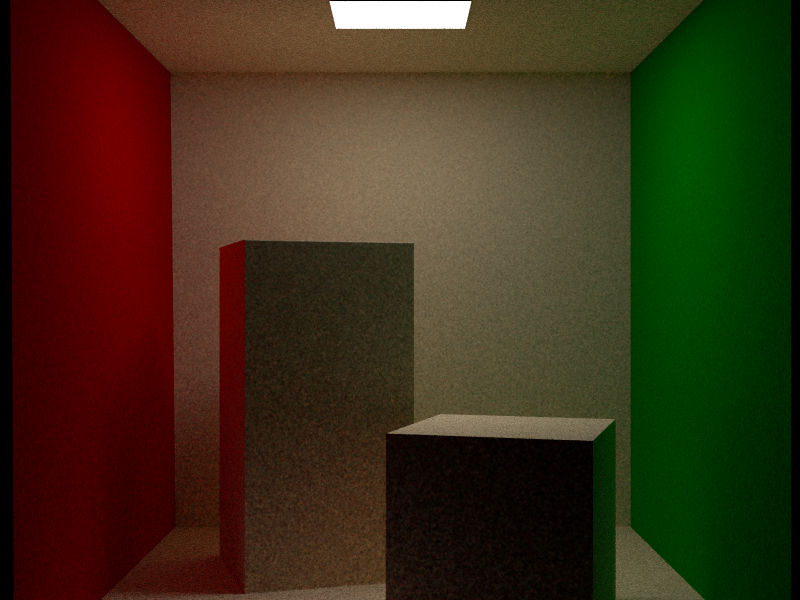
\includegraphics[width=\linewidth]{cornell}
    \caption{cornell \label{fig:cornell}}
  \end{subfigure}%
  \begin{subfigure}[b]{.33\textwidth}
    \centering
    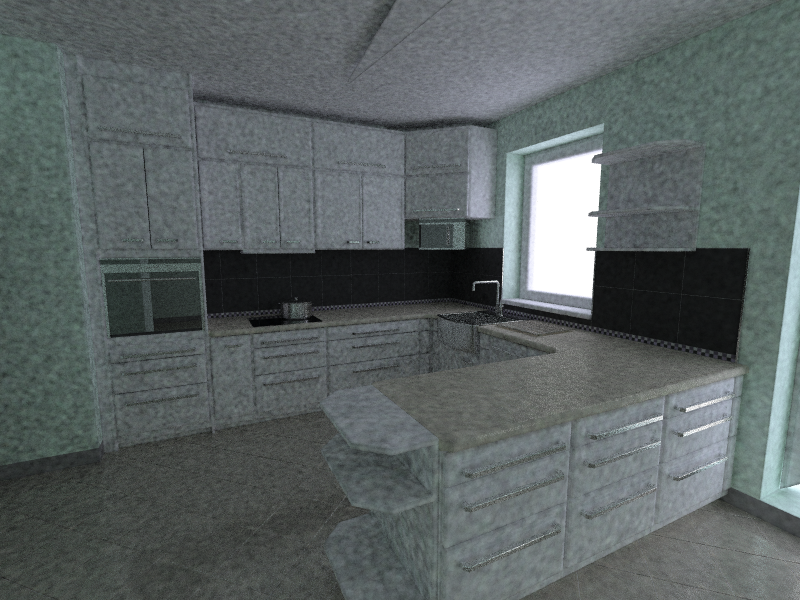
\includegraphics[width=\linewidth]{kitchen}
    \caption{kitchen \label{fig:kitchen}}
  \end{subfigure}%
  \begin{subfigure}[b]{.33\textwidth}
    \centering
    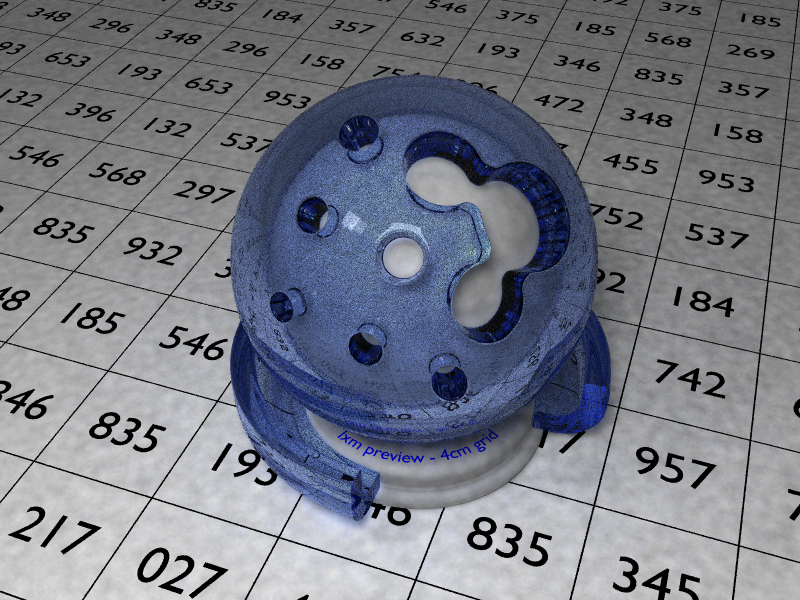
\includegraphics[width=\linewidth]{luxball}
    \caption{luxball \label{fig:luxball}}
  \end{subfigure}
  \caption{Input scenes \label{fig:scenes}}
\end{figure}

\end{document}
